\documentclass{beamer}
\usepackage{graphicx}
\usepackage{url}

\mode<presentation> {
\usetheme{Madrid}
}

\title[LaTeX day 1]{Using \LaTeX{} in SageMathCloud (day 1 of 3)}
\author{William Stein}
\institute[UW]{University of Washington}
\date{April 18, 2016}

\begin{document}

\begin{frame}
\titlepage
\end{frame}



\begin{frame}
\frametitle{Today's Plan}
\begin{block}{What we will do today}
    \begin{enumerate}
    \item Remind me to turn on the screencast; also, peer grading and new homework!
    \item DDoS of SageMathCloud on Friday.
    \item SageMathCloud \LaTeX{} Tutorial
    \end{enumerate}
\end{block}
\end{frame}

\begin{frame}[fragile]
\frametitle{Distributed Denial of Service Attack on Friday}
\begin{block}{DDoS}
    \begin{enumerate}
    \item Wordpress pingback attack. Wrecked our class.  Wrecked my weekend.
    \item Now SMC uses \url{https://www.cloudflare.com/}.
    \end{enumerate}
\end{block}
\begin{center}
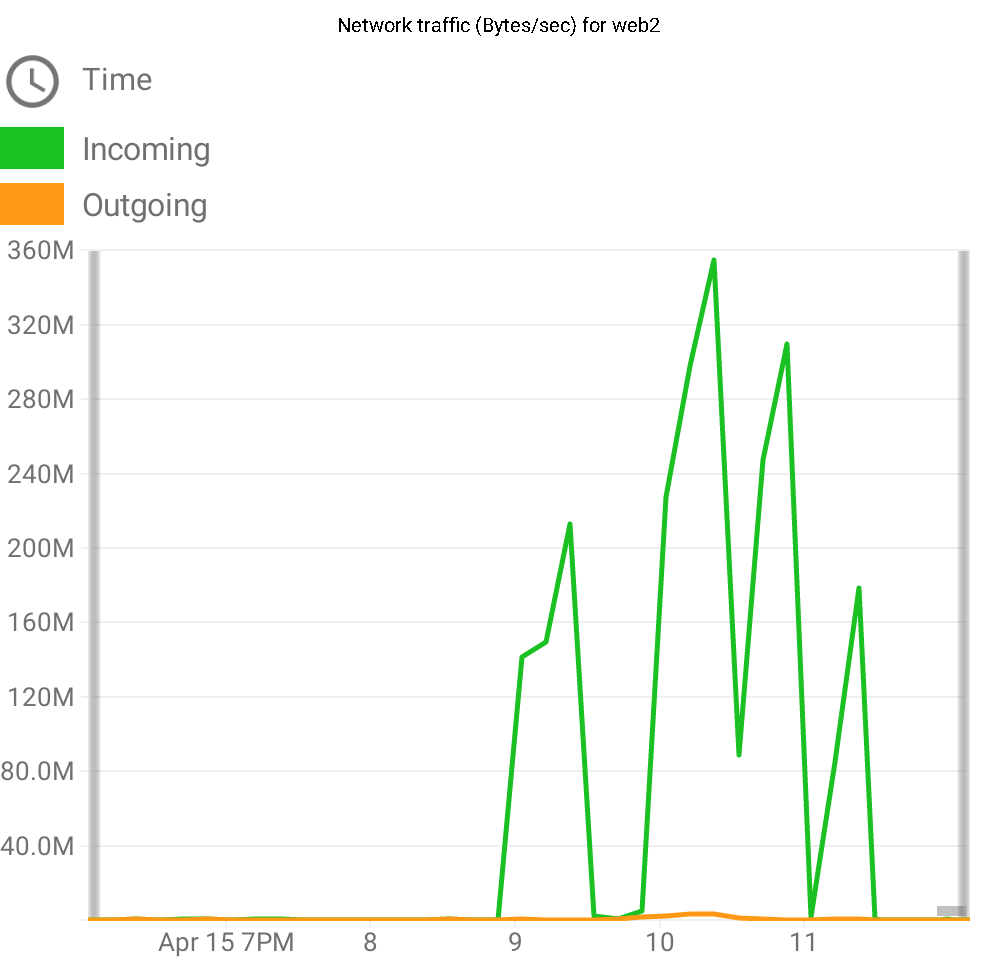
\includegraphics[width=.5\textwidth]{chart-NETWORK-542068901}
\end{center}
\end{frame}

\begin{frame}
\frametitle{General Remarks about \LaTeX{}}
\begin{block}{\LaTeX{}...}
\begin{enumerate}
\item Create professional quality documents involving mathematics.
\item Completely open source and free.  You can install it anywhere.
\item SageMathCloud is one (of many) ways to use it.
\end{enumerate}
\end{block}
\end{frame}

\begin{frame}
\frametitle{\LaTeX{} Tutorial: first steps}
\begin{block}{Do the following}
\begin{enumerate}
\item Create a new blank latex document.
\item Edit it, changing the title and your name, and seeing the result to the right.
\item Find a random math-related wikipedia article, and copy/paste a paragraph of text into your document (this shouldn't work too well, but gives you some math to play with).
\item Try out forward and inverse search.
\item Make errors and see them listed under issues.
\item Download the PDF.
\item Click build, then latex to see the output.
\item Change preview zoom and resolution.
\end{enumerate}
\end{block}

\end{frame}

\begin{frame}[fragile]
\frametitle{\LaTeX{} Tutorial: next steps}
\begin{block}{Do the following}
\begin{enumerate}
\item In your document, type some formulas surrounded by dollar signs.  Try each of the following and some variations on them:
\item \verb|$x^3$|
\item \verb|$\sin(x^\pi)$|
\item \verb|$e^{2\pi i}$|
\item \verb|$\frac{2}{3 + x}$|
\item \verb|$1 + 2 + \cdots + n$|
\item \verb|$\sum_{i=1}^{n} i$|
\item \verb|$\int_{0}^{\pi} \sin(x)$|
\item \verb|$\sqrt{x^3 + 2}$|
\end{enumerate}
\end{block}
\end{frame}


\begin{frame}[fragile]
\frametitle{\LaTeX{} Tutorial: sagetex}
\begin{block}{Do the following}
\begin{enumerate}
\item Put \verb|\usepackage{sagetex}| in the {\bf preamble} of your
latex document. This means put it after \verb|\documentclass...| and before \verb|\begin{document}|.

\item Try typing this formula in: \verb|$2018 = \sage{factor(2018)}$|.

\item Once that works, try
some things from \url{http://mirrors.ibiblio.org/CTAN/macros/latex/contrib/sagetex/sagetexpackage.pdf}

\item \verb|\sageplot[width=.7\textwidth]{plot(sin,0,1)}|

\end{enumerate}
\end{block}
\end{frame}


\end{document}

